%%%%%%%%%%%%%%%
% This file is concerned with the system sequence diagram,
% a subsection of the functional requirements.
%
% Please remember to compile the document from "00_finalreport.tex".
% It will not work otherwise.
%%%%%%%%%%%%%%%

	\subsection{System Sequence Diagram}
	
		\subsubsection{Diagram}
			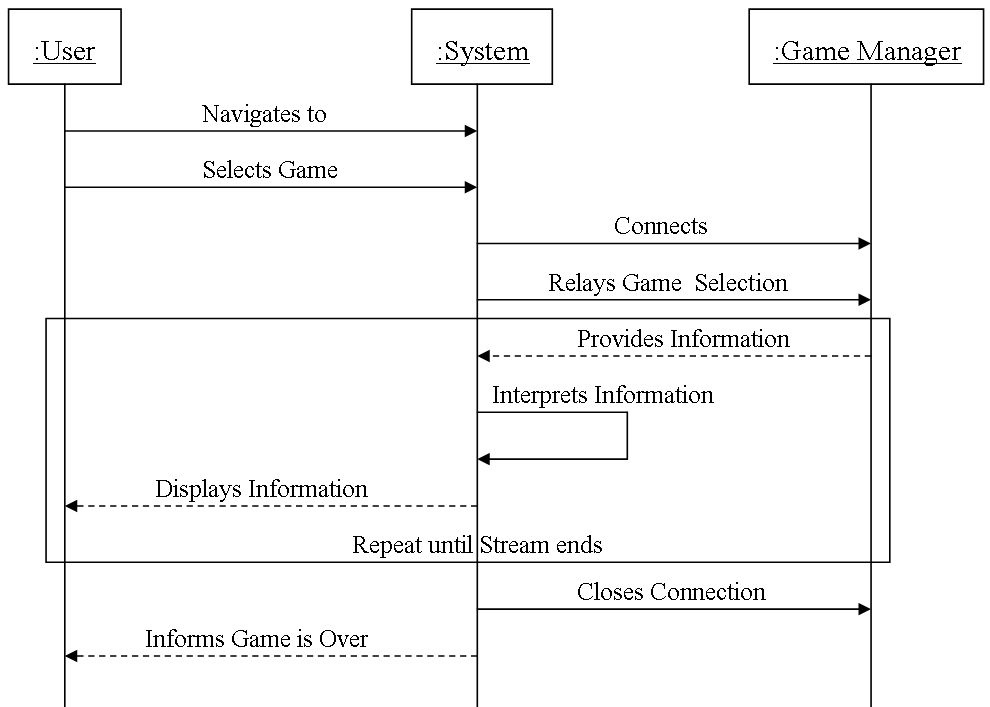
\includegraphics[width=1.0\textwidth]{./SSD_of_Watch_Live.png}
			
		\subsubsection{Description}
			Within our System Sequence Diagram, we have three actors: the User, the System, and the Game Manager. The User navigates to the game selection and selects a game to watch from the System, and the System connects to the Game Manager. The System then informs the Game Manager which game the user has selected. With a game selected, the Game Manager will provide game information to the System. The System will interpret the game information and then display this information to the User. These three steps will be repeated until the stream of game information ends. At this point, the System will close the connection with the Game Manager. Once the connection is closed, the System will notify the User that the current game is now over.
